\subsection{Theory}
The K-Nearest Neighbour (K-NN) method is in this report used to classify a unknown digit to a set of known digits ranging from zero to nine.
%The data is split into two groups: One is for training and one is for testing. 
A set of the $k$ nearest neighbour is found using the euclidean distance to the pixel values in a training set of which the elements are already classified.
The result from the classification is found by counting the number of occurrences from the set of the $k$ nearest neighbours and choosing the most prominent.

%To see how this method performs a multitude of tests are performed to see how multiple parameters affect the success rate and the speed.

An example of such is seen in figure \ref{fig:knn_illustration}.

\begin{figure}[H]
\centering
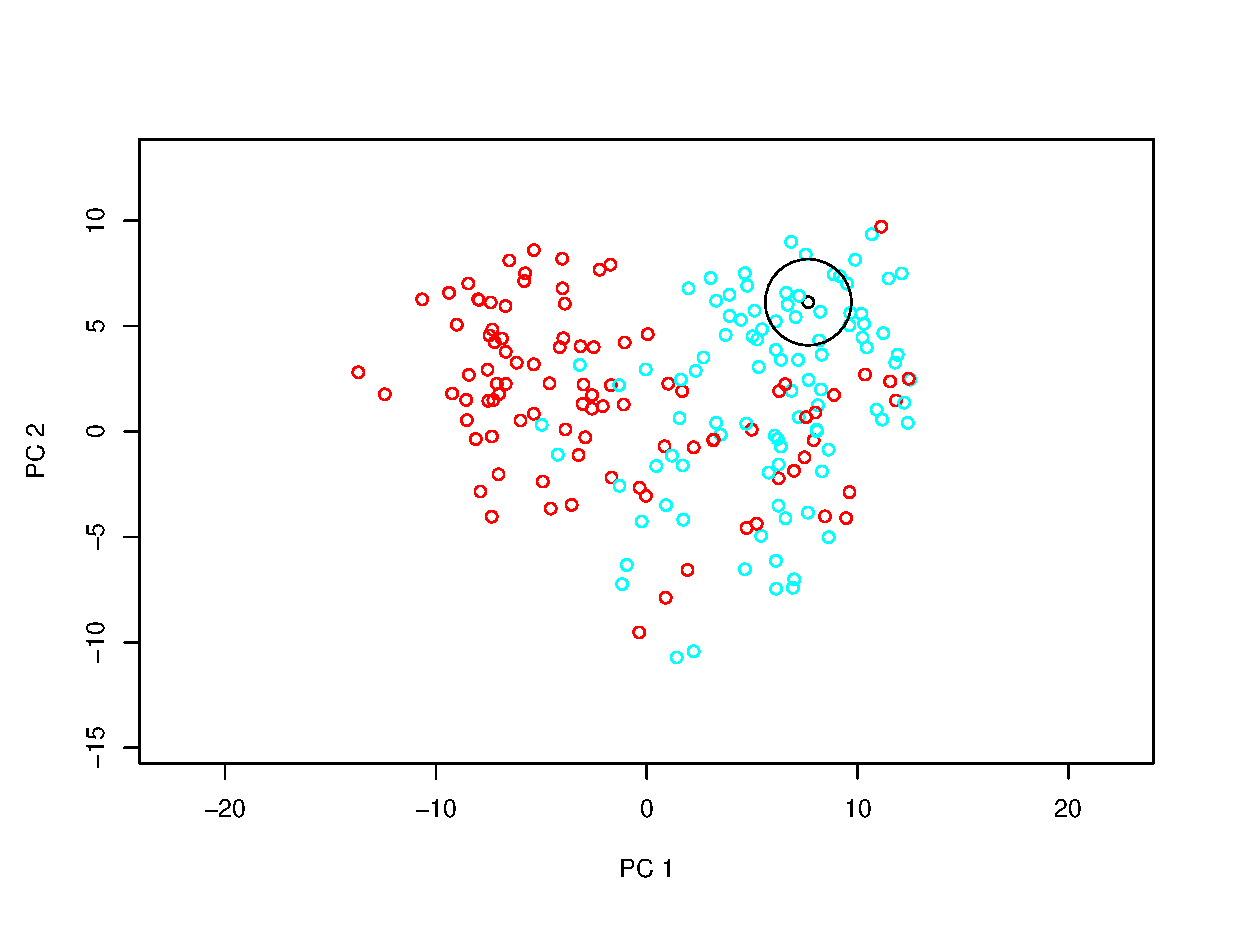
\includegraphics[width = 0.8 \textwidth]{graphics/knn_vis}
\caption[Visualization of the K-NN approach.]{Illustration of the K-NN approach with $k = 10$ on the normalized data for two classes plotting the two most prominent principle components.}
\label{fig:knn_illustration}
\end{figure}

In figure \ref{fig:knn_illustration} the black data point is an element of the blue test set.
The circle around it encircles the ten nearest neighbours.
Since there are more blue neighbours within the circle than red, then the classification in this case correctly classifies the element to the blue one.

